\chapter{Оценка характеристик метода на избранных тестовых проектах}

Для подтверждения характеристик метода анализа было создано три тестовых проекта.
Проекты были созданы исходя из следующих критериев:
\begin{itemize}
    \item использование нескольких популярных языков в одном проекте,
    \item каждый проект решает задачу в определенной уникальной предметной области,
    \item используемые языки должны представлять различные парадигмы программирования,
    \item каждый из проектов должен вовлекать различные сценарии использования LSP.
\end{itemize}

В перечисленных примерах используются рисунки для визуализации графа областей, а именно рисунки \ref{fig:example_1}, \ref{fig:example_2} и \ref{fig:example_3}.
Для данных рисунков принято следующее соглашение: розовыми линиями отмечается отношение <<определяет>>, синими -- <<ссылается>>, красными -- <<имеет
общую область видимости>>, зелеными -- <<проистекает>> или <<следует>> (в случае анализа DFG).
Некоторые идентификаторы имеют соответствующие плашки с присвоенными типами.

Все полученные ограничения находятся в открытом репозитории проекта в виде файлов кода на языке TypeScript. \footnote{https://github.com/UberDever/crosslingual-analysis/tree/master/projects/crossy/lsp-adapter/examples}

\section{Пример 1 -- C\# и Visual Basic}

\subsection{Общее описание}

Приложение, реализованное на C\# использует слой взаимодействия на уровне байткода IL и имеет в зависимостях библиотеку,
реализованную на Visual Basic. Весь проект объединен через Solution файл. Такой сценарий часто встречается
в legacy приложениях, при переходе кодовой базы с Visual Basic на C\#.

Основной проблемой в проекте является отсутствие информации о том, где конкретно объявлен класс на другом языке и какие поля он содержит.

Вовлекаемые языки: C\#, Visual Basic, XML (\texttt{.sln}, \texttt{.vbproj} и \texttt{.csproj} файлы).
Предположительные предметные области: Энтерпрайз приложения, частные коммерческие решения.
Рассмотренные парадигмы языков: ООП, структурированные данные.

\subsection{Окружение}

При извлечении кода могут быть использованы файлы проектов \texttt{.vbproj} и \texttt{.csproj}, в дальнейшей
достаточно построение <<слепка>> файловой структуры проекта.

\subsection{Трансляция и решение}

Трансляция может вовлекать в себя стандартный reaching definition анализ \cite{static-program-analysis} и прямое отображение
статической структуры классов и объектов на ограничения графов областей. При отображении не были использованы
структурные предикаты, так как структура модулей и классов C\# не имеет определенной семантики в отношении
типов и возможной вложенности. 

Полученный граф областей вкупе с типовыми ограничениями представлен на рисунке \ref{fig:example_1}.
\begin{figure}[H]
    \centering
    \resizebox{1\linewidth}{!}{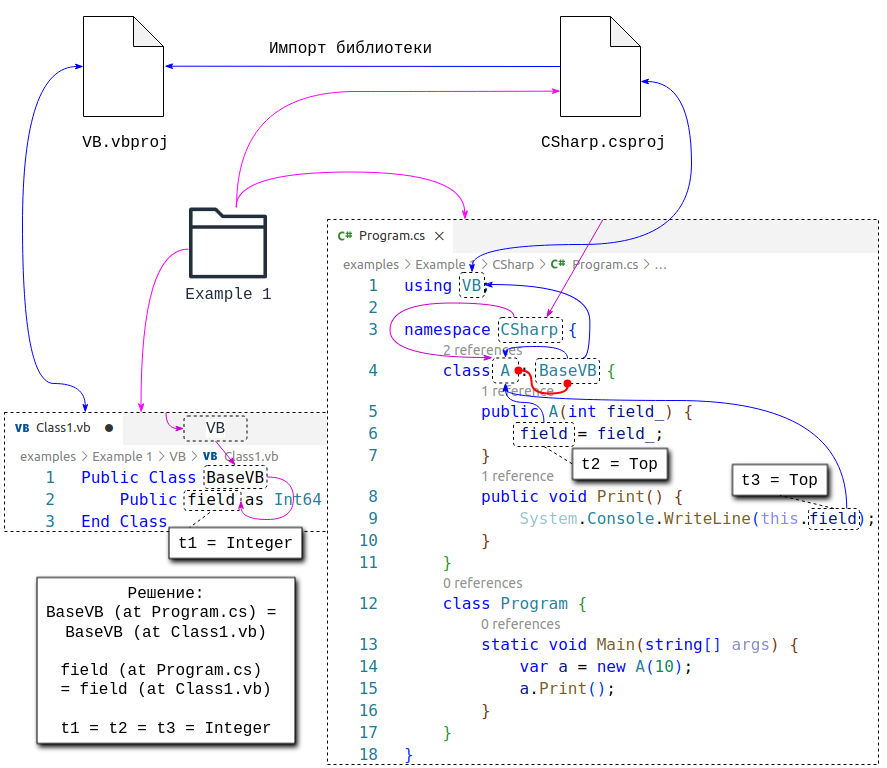
\includegraphics[height=1\textheight]{inc/img/example_1}}
    \caption{Визуализация графа областей и типовых ограничений для примера 1}
    \label{fig:example_1}
\end{figure}

\subsection{Онтология}

Типы, добавленные в онтологию:
\begin{itemize}
    \item Integer -- целочисленное число неспецифицированной точности,
    \item Top -- супертип всех возможных типов, также является маркером отсутствия информации об идентификаторе.
\end{itemize}

\subsection{Сценарии LSP}

Для данного примера было решено реализовать два сценария использования, характерных для ООП языков: <<Type hierarchy>> 
(получение иерархии типов) и <<Go to definition/declaration>> (перейти к объявлению/использованию).
Предполагаемые примеры внешнего вида реализации таких сценариев показаны на рисунке \ref{fig:lsp-type-hierarchy} и рисунке \ref{fig:lsp-goto}
соответственно.

\begin{figure}[H]
    \centering
    \resizebox{1\linewidth}{!}{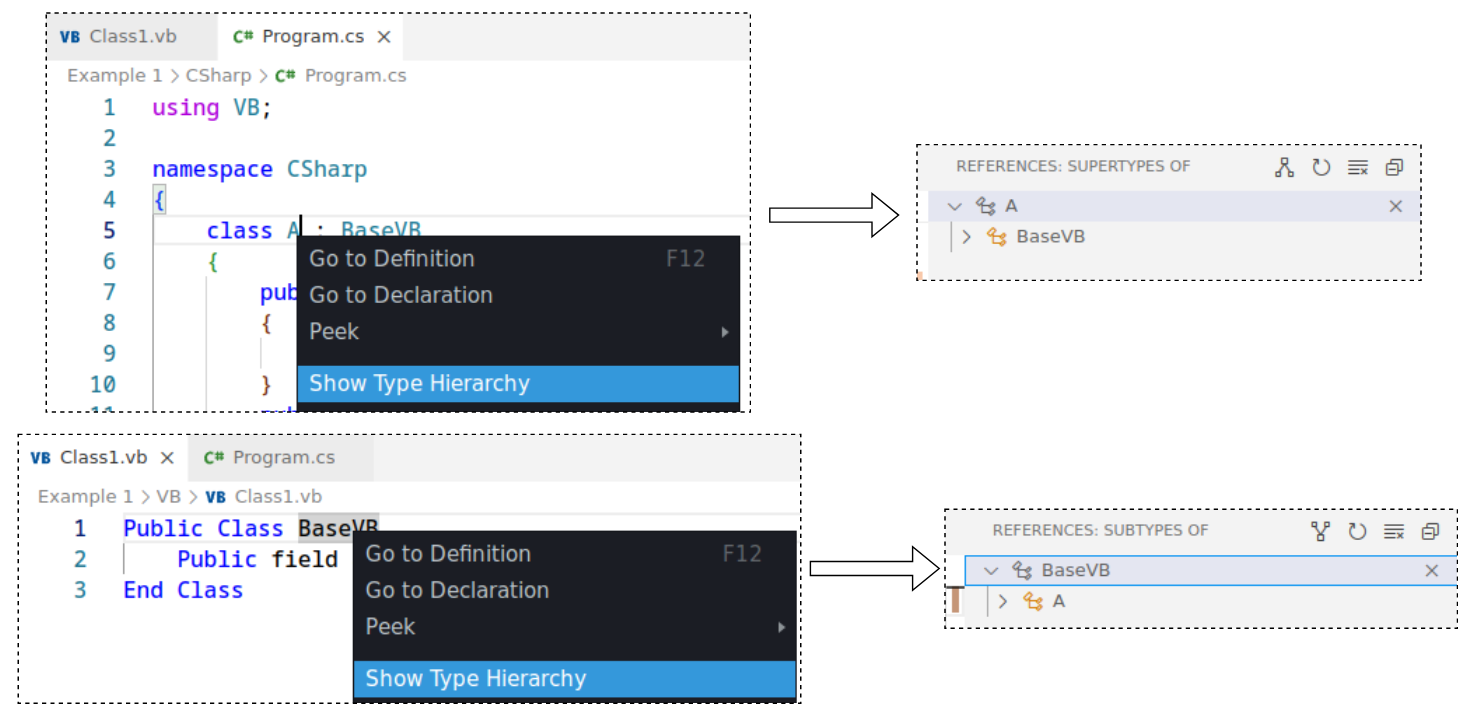
\includegraphics[height=1\textheight]{inc/img/lsp-type-hierarchy}}
    \caption{Сценарий LSP <<Type hierarchy>>}
    \label{fig:lsp-type-hierarchy}
\end{figure}

\begin{figure}[H]
    \centering
    \resizebox{1\linewidth}{!}{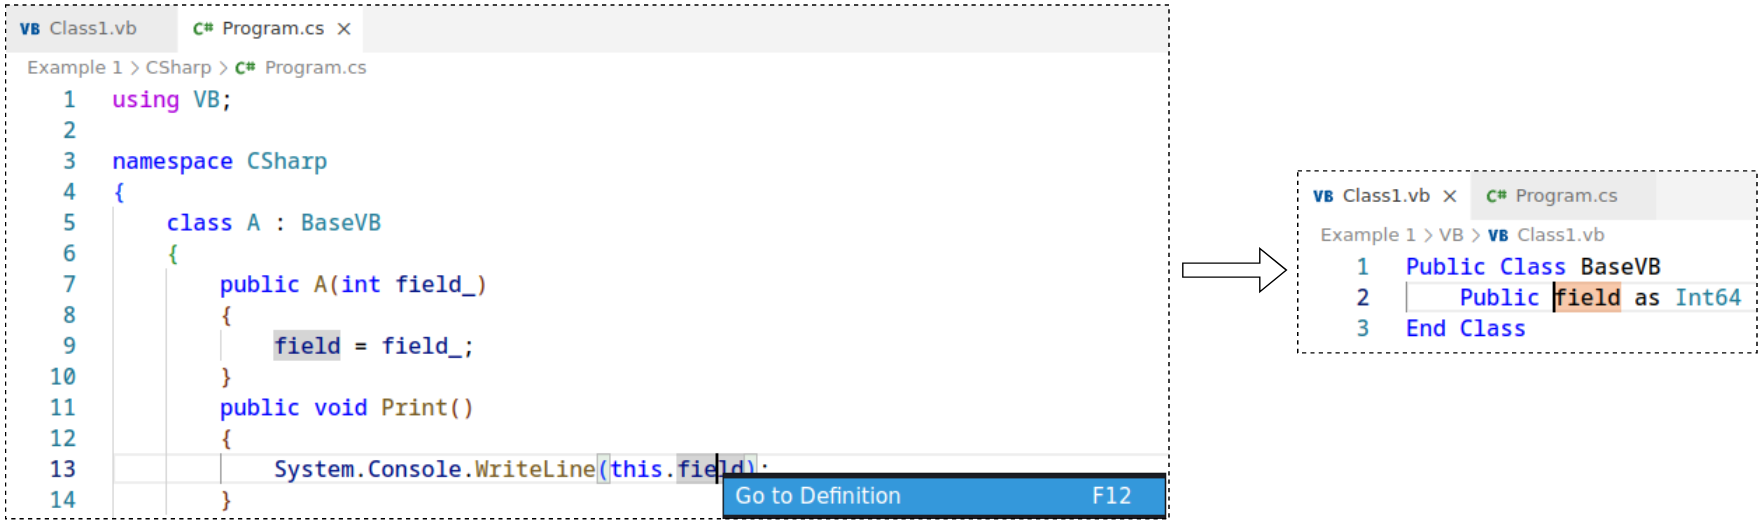
\includegraphics[height=1\textheight]{inc/img/lsp-goto}}
    \caption{Сценарий LSP <<Go to definition/declaration>>}
    \label{fig:lsp-goto}
\end{figure}

\section{Пример 2 -- С++, Python 3 и Shell}

\subsection{Общее описание}

Проектом служит библиотека, реализованная на C++ и предназначенная для задач научных вычислений. Для этой
библиотеки разработана небольшая инфраструктура в виде скриптов командной оболочки для сборки и запуска тестирования библиотеки.
Также, для библиотеки реализован тестовый фреймворк в виде отдельного скрипта на Python 3.

Основной проблемой в проекте является отсутствие информации о сигнатурах функций, экспортируемых такой библиотекой.

Вовлекаемые языки: C++, Python 3, Shell.
Предположительные предметные области: Научные вычисления, DevOps и тестирование, машинное обучение.
Рассмотренные парадигмы языков: Динамические языки, процедурные языки, языки командной оболочки.

\subsection{Окружение}

В данном проекте используются стандартные BusyBox утилиты (\texttt{rm, mkdir, mv} и т.д.), а также
компилятор \texttt{c++}. Информация об этих инструментах может быть использована при анализе зависимостей
с соответствующей выдачей отчета об ошибках, однако в данном примере такая информация не анализируется.
Анализатором Shell используется знание о принципе работы флагов компилятора \texttt{c++}, что также частично
является информацией из окружения (так как флаги могут зависить от, например, версии компилятора).

\subsection{Трансляция и решение}

В данном примере использован интенсивный внутренний анализ графа потока данных, для выявления точек (а точнее, идентификаторов), которые
потенциально взаимодействуют на межъязыковом уровне. Так, например, для кода Python 3 была выявлена связь идентификатора \texttt{lib\_dir/lib.so}
и всех функций, которые брались из соответствующей библиотеки. Также, при анализе Shell из информации о принципе работы компилятора \texttt{c++}
удается вывести, что файлы \texttt{lib.cpp} и \texttt{lib.so} имеют общую область видимости в отношении идентификаторов, которые ими экспортируются.

Полученный граф областей вкупе с типовыми ограничениями представлен на рисунке \ref{fig:example_2}.
\begin{figure}[H]
    \centering
    \resizebox{1\linewidth}{!}{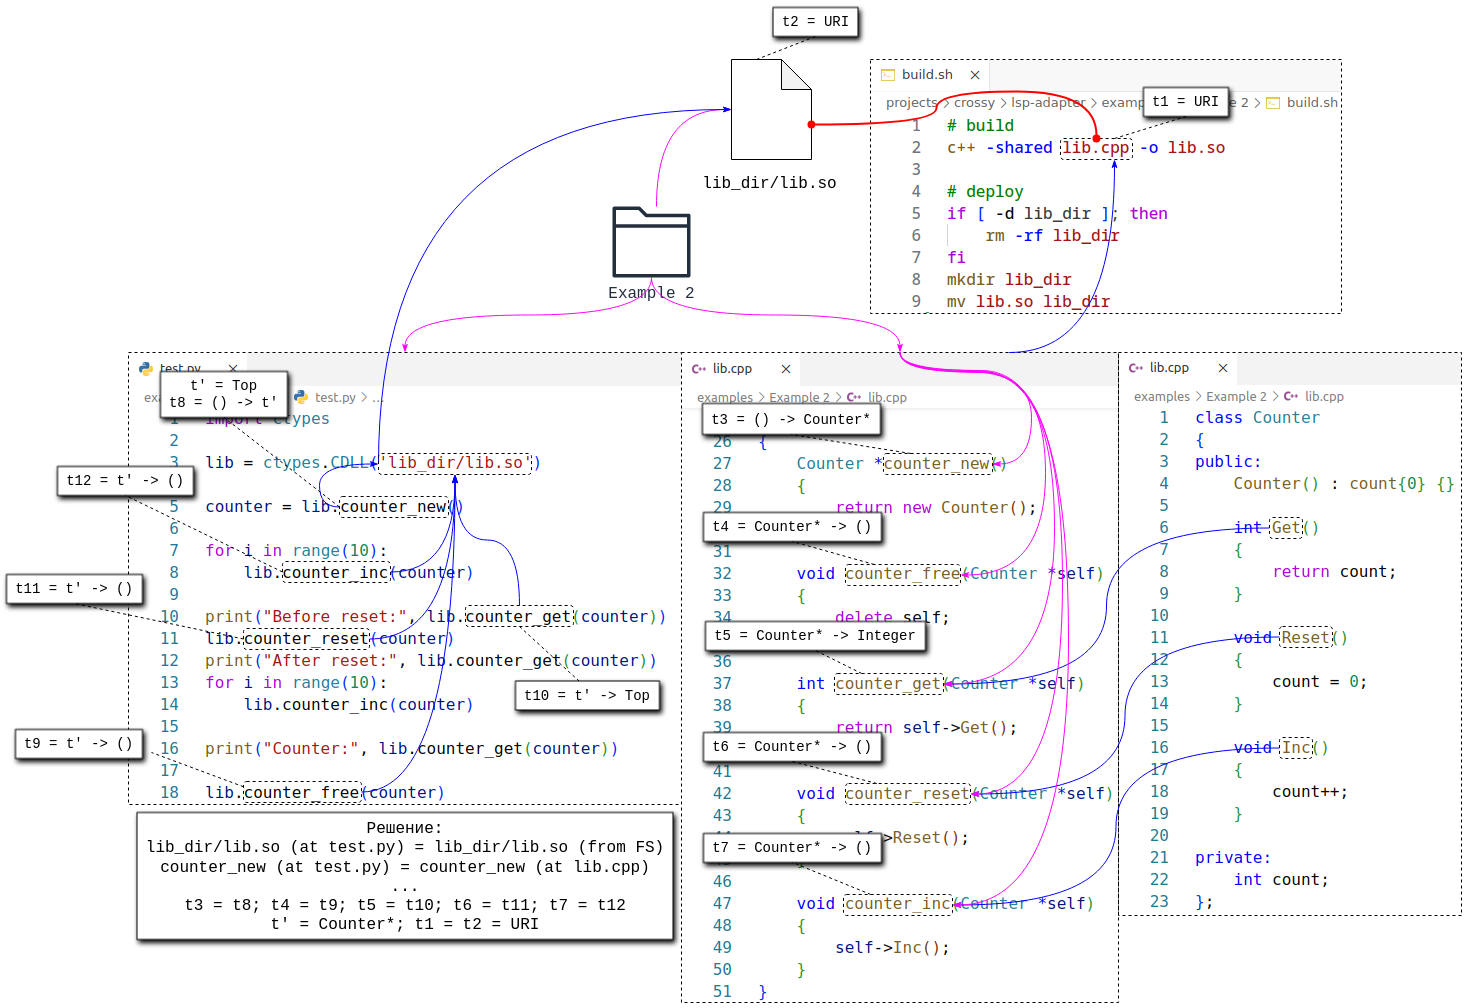
\includegraphics[height=1\textheight]{inc/img/example_2}}
    \caption{Визуализация графа областей и типовых ограничений для примера 2}
    \label{fig:example_2}
\end{figure}

\subsection{Онтология}

В онтологию был добавлен структурный предикат <<библиотека>>: в сущности, библиотекой может считаться
идентификатор, имеющий тип \texttt{URI} и имеющий связанную область видимости. В данной области видимости
могут быть объявлены идентификаторы имеющие только функциональный тип и не имеющие вложенных областей видимости.
Такой предикат позволяет моделировать простейшие библиотеки на языке C, с отсутствием внешних глобальных переменных, что
может быть характерно для определенных проектов.

\subsection{Сценарии LSP}

Так как для данного проекта важна информация о сигнатурах функций библиотеки, решено было реализовать два поддерживающих
разработчика сценария: <<Completion>> (автодополнение) и <<Signature help>> (подсказка сигнатуры).
Предполагаемые примеры внешнего вида реализации таких сценариев показаны на рисунке \ref{fig:lsp-autocomplete} и рисунке \ref{fig:lsp-signature}
соответственно.

\begin{figure}[H]
    \centering
    \resizebox{1\linewidth}{!}{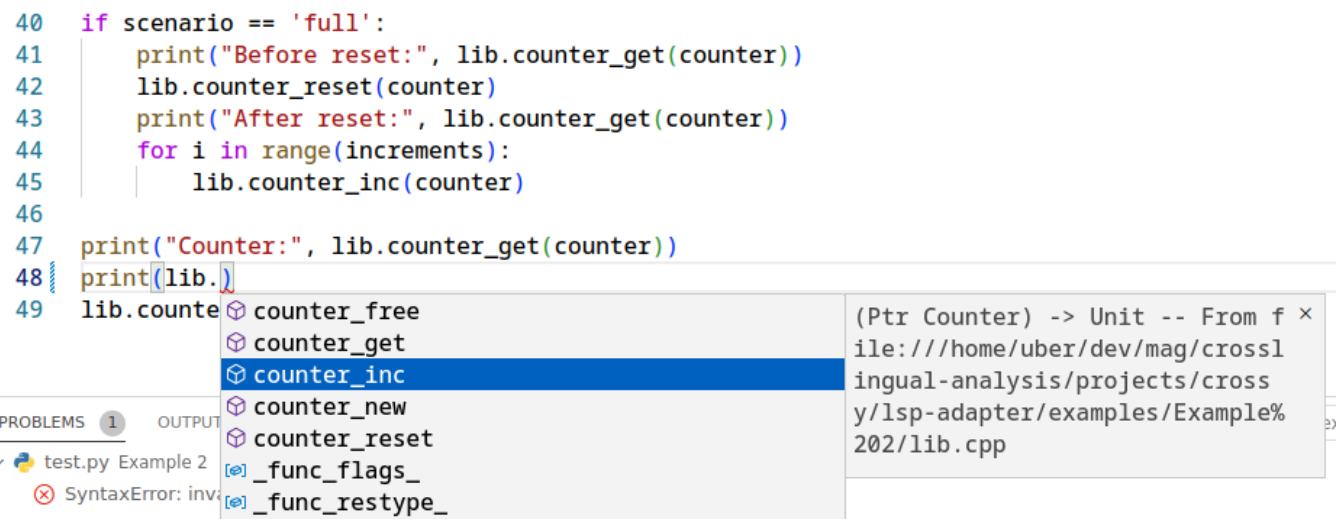
\includegraphics[height=1\textheight]{inc/img/lsp-autocomplete}}
    \caption{Сценарий LSP <<Completion>>}
    \label{fig:lsp-autocomplete}
\end{figure}

\begin{figure}[H]
    \centering
    \resizebox{1\linewidth}{!}{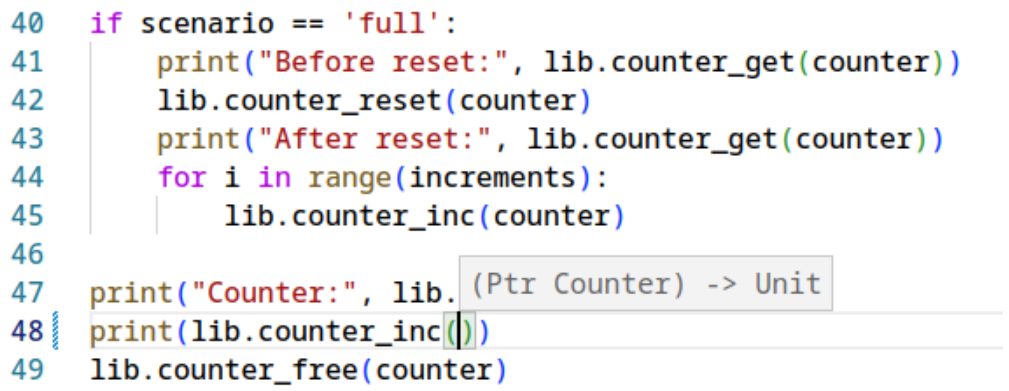
\includegraphics[height=1\textheight]{inc/img/lsp-signature}}
    \caption{Сценарий LSP <<Signature help>>}
    \label{fig:lsp-signature}
\end{figure}

\section{Пример 3 -- Golang и JavaScript}

\subsection{Общее описание}

Проект представляет собой простейшее фуллстак веб-приложение, с двунаправленным взаимодействием
между клиентом и сервером. Клиентом выступает браузер, который подгружает HTML страницу и соответствующий JavaScript
код для обеспечения интерактивности такой страницы. Сервер реализован на Golang и является стандартным
HTTP сервером, обеспечивающи обмен данными посредством JSON. Таким образом, проект представляет стандартное
приложение, использующее Rest API.

Сервер имеет внутреннее состояние, которое изменяется при соответствующих запросах с веб-страницы. Клиент, в свою
очередь, обновляет состояние веб-страницы при ответе сервера.

Основной проблемой проекта является неявная связь между сетевыми путями сервера и клиента, а также
отсутствие выраженной схемы данных, которыми они обмениваются.

\subsection{Окружение}

В данном проекте не используется явное окружение, однако серверу требуется сетевой порт для возможности
запуска и отправки сообщений. Такая информация не используется в анализе, так как она имеет небольшую применимость.

\subsection{Трансляция и решение}

Анализ данного проекта является самым сложным из всех перечисленных примеров. Это связано с тем, что
проекты, использующие взаимодействие по сети, имеют специализированные библиотеки и фреймворки, а
уровень таких библиотек достаточно высоким и вовлекающим большое количество различных компонентов.
В данном случае, при анализе сервера Golang потребуется вывести собственную структуру подграфа, обозначающую
веб-сервер. Используя интенсивный анализ потока данных, получается использовать эту структуру
для инкапсуляции ключевых особенностей веб-сервера -- наличие определенных путей, которые
могут содержать информацию при применении различных запросов к ним (HTTP.GET или HTTP.POST).

Такая структура (или <<идея>>) веб-сервера также ожидается и на стороне клиента, так как
доступ к определенным путям возможен только при соблюдении определенного протокола взаимодействия (в данном случае HTTP и Rest API).

Помимо этих особенностей, веб-сервер имеет определение типа данных, передаваемых по сети, с автоматически генерируемой
структурой (через использование тегов структур \cite{struct-tags}). Такая информация является очень специфической и требует
серьезного знания того, как используются теги структур от анализатора. Тем не менее, извлечение такой информации
возможно и её отображение в граф областей допустимо.

Полученный граф областей вкупе с типовыми ограничениями представлен на рисунке \ref{fig:example_3}.
\begin{figure}[H]
    \centering
    \resizebox{1\linewidth}{!}{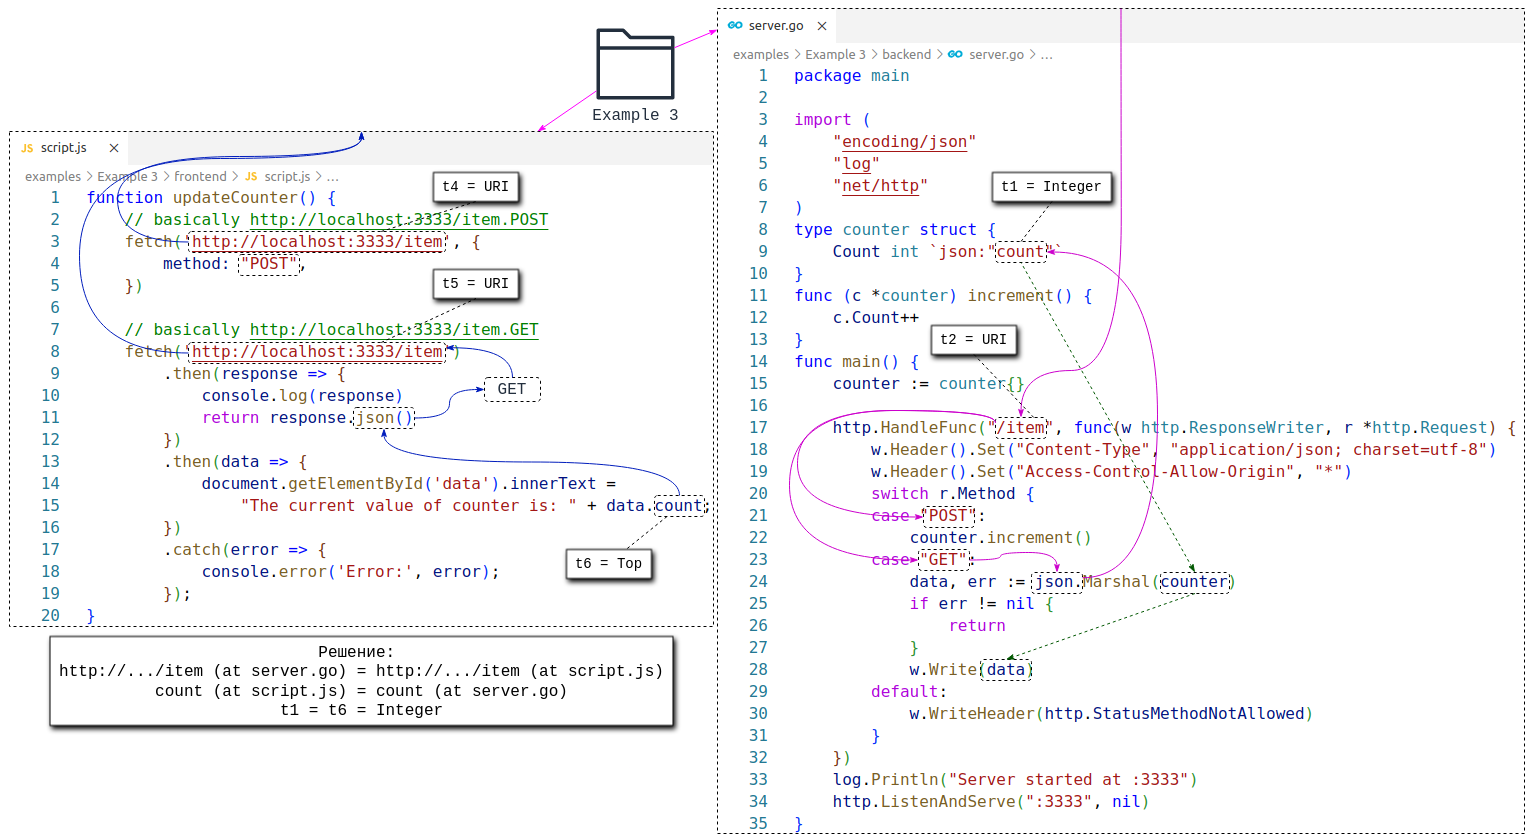
\includegraphics[height=1\textheight]{inc/img/example_3}}
    \caption{Визуализация графа областей и типовых ограничений для примера 3}
    \label{fig:example_3}
\end{figure}

\subsection{Онтология}

В дополнение к рассмотренным типам, в онтологию вошли новые типы:
\begin{itemize}
    \item Numeric -- числовой тип неопределенного размера и точности (рациональное число),
    \item Bool -- булевый тип,
    \item String -- строка в случайной кодировке, исходящей из принятых в проекте,
    \item Unit -- тип, населенный единственным значением.
\end{itemize}

Был добавлен структурный предикат <<веб-сервер>> для протокола HTTP. Для такого предиката выполняется ряд
общих для веб-серверов условий: такой сервер должен быть представлен URI, он обязан иметь поля \texttt{GET, POST} и иные (в зависимости
от проекта), а также такие поля должны содержать данные в определенном формате (в данном случае JSON). Также был добавлен предикат
<<JSON-объект>>, допускающий любой уровень вложенности областей видимости, но ограничивающий типы, присваиваемые идентификаторам (только
Numeric, Bool, Unit, String).

\subsection{Сценарии LSP}

Для упрощения поддержки согласованности проектов между собой решено было реализовать
два сценария: <<Rename symbol>> (переименование символа под курсором) и <<Document diagnostics>> (диагностика документа).
Предполагаемые примеры внешнего вида реализации таких сценариев показаны на рисунке \ref{fig:lsp-rename} и рисунке \ref{fig:lsp-diagnostics}
соответственно.

\begin{figure}[H]
    \centering
    \resizebox{1\linewidth}{!}{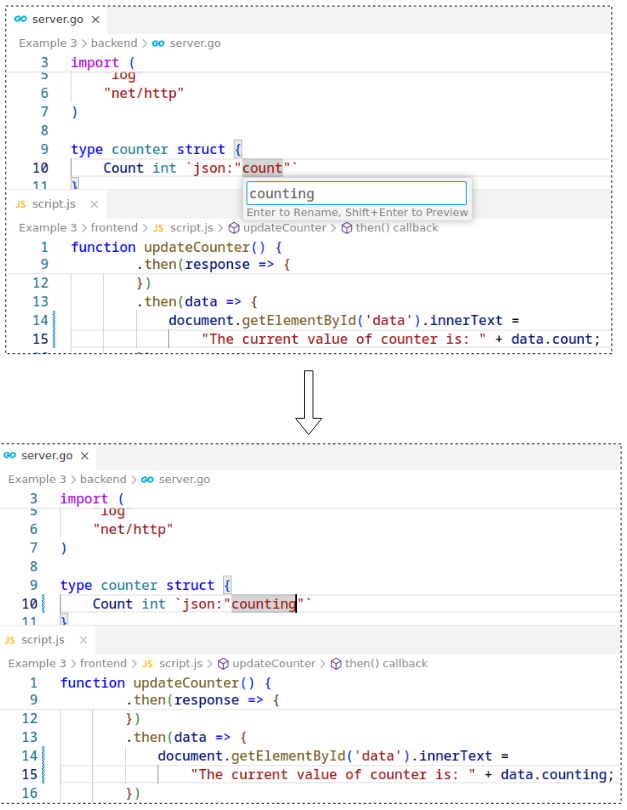
\includegraphics[height=1\textheight]{inc/img/lsp-rename}}
    \caption{Сценарий LSP <<Rename symbol>>}
    \label{fig:lsp-rename}
\end{figure}

\begin{figure}[H]
    \centering
    \resizebox{1\linewidth}{!}{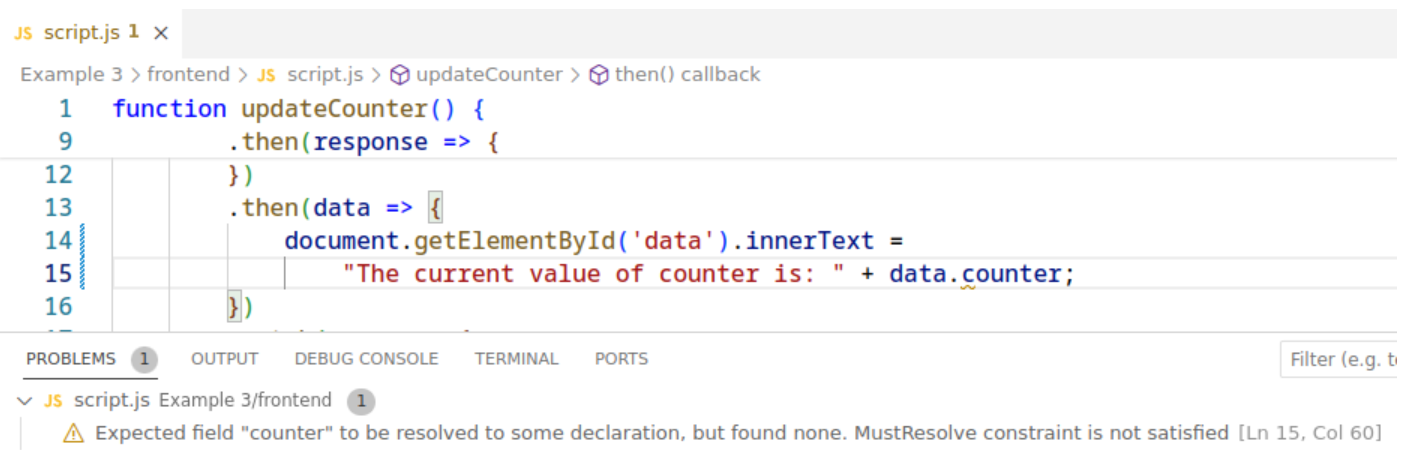
\includegraphics[height=1\textheight]{inc/img/lsp-diagnostics}}
    \caption{Сценарий LSP <<Document diagnostics>>}
    \label{fig:lsp-diagnostics}
\end{figure}

\section{Анализ поддержки описанных сценариев в существующих инструментальных средствах}

Для сравнительной оценки возможностей разработанного анализатора (и созданного метода) были рассмотренны соответствующие
возможности современных инструментальных средств, а именно IDE. Выборка средств происходила исходя из индекса популярности
существующих IDE \cite{top-ide}. Так как рассмотренные примеры проектов используют различные языки, решено было
выбрать наиболее подходящие IDE, исходя из позиции в рассматриемом списке.

Сравнительный анализ IDE и разработанного анализатора представлен в таблице \ref{ide-comparison}.
\begin{table}[H]
    \caption{\textbf{Сравнение существующих IDE и анализатора}}
    \resizebox{1 \textwidth}{!}{\begin{tabular}{|p{4cm}|p{7cm}|p{7cm}|}
    \hline \textbf{Средство} & \textbf{Преимущества в сравнении с анализатором} & \textbf{Недостатки в сравнении с анализатором} \\ 
    \hline Visual Studio 2022 + ReSharper & Поддержка большего количества сценариев LSP,
    поддержка описанных сценариев (<<Go to definition/declaration>>, <<Type hierarchy>>),
     поддержка рефакторингов на основе более полного семантического представления & 
     Проприетарное, платное решение; ограниченная поддержка различных языков (3 основных и несколько DSL),  \\
    \hline Visual Studio Code (плагины Golang и JavaScript) & Бесплатное, открытое решение; Хорошая интеграция
    с инструментарием как Golang, так и JavaScript &
    Отсутствие поддержки описанных сценариев (<<Rename symbol>>, <<Document diagnostics>>), слабая поддержка языкоспецифичных особенностей
    (например, анализ путей веб-сервера для Golang) \\
    \hline Clion 2023.1 & Поддержка основных систем сборки для C++ (cmake, make), поддержка большего количества сценариев LSP
    для C++ & 
    Проприетарное, платное решение; Отсутствие поддержки описанных сценариев (<<Completion>>, <<Signature help>>),
    плохая совместимость с Python (только посредством плагина) \\
    \hline Visual Studio Code (плагины С++ и Python) & Бесплатное, открытое решение; Широкий
    набор инструментов для Python &
    Отсутствие поддержки описанных сценариев (<<Go to definition/declaration>>, <<Type hierarchy>>) \\
    \hline
    \end{tabular}}\label{ide-comparison}
\end{table}

Как видно из таблицы, на данный момент не существует средств, реализующих функциональность разработанного мультиязыкового
анализатора в полной мере. Расширение ReSharper реализует все сценарии LSP на мультиязыковом уровне, но
его поддержка ограничена лишь тремя языками (C\#, Visual Basic, F\#). Остальные средства не 
производят выявления межъязыковых связей обычно по двум причинам: либо средство слишком универсально
(Visual Studio Code), либо слишком специализировано (Clion).

Таким образом, разработанный анализатор является наиболее полным в отношении
поддерживаемых мультиязыковых сценариев LSP, что подтверждает работоспособность
метода и удовлетворяет выдвигаемые к нему требования.

\clearpage
